\documentclass[crop,tikz]{standalone}
\usepackage{amsmath,amssymb}
\usepackage{pgfplots}

\definecolor{cliquecolor}{HTML}{457B9D}
\newcommand{\cliquecolor}{cliquecolor!75!blue}
\definecolor{cyclecolor}{HTML}{CC5800}
\newcommand{\cyclecolor}{cyclecolor!75!red}
\definecolor{othercolor}{HTML}{4E7E67}
\newcommand{\othercolor}{othercolor!75!green}

\begin{document}
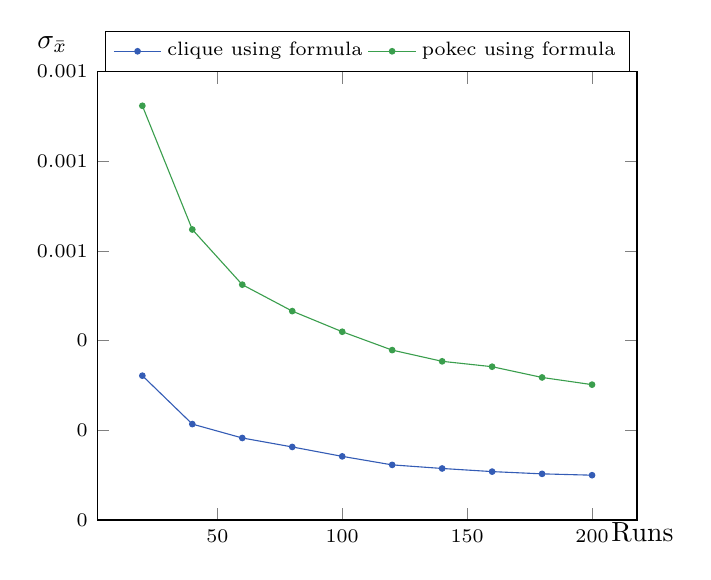
\begin{tikzpicture}
  \pgfplotsset{yticklabel style={/pgf/number format/fixed, /pgf/number format/precision=3}, scaled y ticks=false}
  \pgfplotsset{every axis legend/.append style={at={(0.5,1)},anchor=south}} %%% To put legend outside the box
\begin{axis}[legend columns=2, %%% Legends horizontally
        %axis equal image=true,unit vector ratio=9 1,width=1.1\columnwidth, %%% size of box
        ymin=0,
        ymax=0.001,
        every tick label/.append style={font=\scriptsize},legend style={font=\scriptsize}, %%% size of legends
        xlabel=Runs, ylabel=$\sigma_{\bar{x}}$, %%% axis labels
        every axis y label/.style={at={(ticklabel cs:1.02)},anchor=south west}, %%%% position of y-axis legend
        every axis x label/.style={at={(ticklabel cs:1.01)},anchor=south}, %%%% position of y-axis legend
        ]
    %\draw[help lines] (axis cs:0,1) -- (axis cs:3,1);
\addplot[color=\cliquecolor,mark=*,mark size=1pt] coordinates {
  (20, 0.000322)
  (40, 0.000214)
  (60, 0.000183)
  (80, 0.000163)
  (100, 0.000142)
  (120, 0.000123)
  (140, 0.000115)
  (160, 0.000108)
  (180, 0.000103)
  (200, 0.000100)
};
\addplot[color=\othercolor,mark=*,mark size=1pt] coordinates {
  (20, 0.000924)
  (40, 0.000648)
  (60, 0.000525)
  (80, 0.000466)
  (100, 0.000420)
  (120, 0.000379)
  (140, 0.000354)
  (160, 0.000342)
  (180, 0.000318)
  (200, 0.000302)
};
\legend{
  clique using formula,
  pokec using formula,
}
\end{axis}
\end{tikzpicture}
\end{document}
